\chapter{General Project Context}
\label{chap:General Project Context}

% ─────────────────────────────────────────────
\section*{Introduction}
\addcontentsline{toc}{section}{Introduction}
% ─────────────────────────────────────────────

I had the opportunity to complete my first internship at Cognitus Corporation, specifically within its Global Delivery and Support Center (GDSC) located in Tangier, Morocco. This experience constituted my very first immersion into the world of enterprise information systems, and more precisely into the SAP ecosystem. In the sections that follow, I will introduce Cognitus Corporation as a global organization, shed light on its Tangier office and its strategic role within the group, and then present the technical project I was entrusted with during this internship period.

\newpage

% ─────────────────────────────────────────────
\section{Cognitus Corporation}
% ─────────────────────────────────────────────

\subsection{About Cognitus Corporation}

\begin{figure}[H]
    \centering
    
\includegraphics[width=12cm]{Figures/logoCognitus.jpg}
    \caption{Cognitus Corporation Logo}
    \label{fig:cognitus_logo}
\end{figure}

Cognitus Corporation is a global SAP Gold Partner and a leading provider of cloud ERP implementations, SAP consulting, and digital transformation services. Founded with the mission of helping organizations unlock the full potential of SAP technology, Cognitus has built over two decades of deep industry expertise across more than eleven verticals, including manufacturing, public sector, retail, healthcare, and financial services.

The company offers a comprehensive range of SAP-centered services, spanning end-to-end implementation of SAP S/4HANA, RISE with SAP, and GROW with SAP programs, as well as specialized consulting in areas such as supply chain optimization, contract lifecycle management (CLM), and real-time billing. In addition to its consulting capabilities, Cognitus has developed a suite of proprietary AI-enabled software assets designed to accelerate data migration, automate compliance workflows in government contracting environments, and streamline business process transformation.

In 2025, Cognitus was acquired by IBM, reinforcing IBM's strategic position in the global SAP services market. This acquisition underscores Cognitus's standing as a recognized leader in RISE with SAP and GROW with SAP advisory, and consolidates its portfolio of accelerators and industry-specific SAP solutions within IBM's broader technology ecosystem.

Throughout its growth, Cognitus has maintained a strong commitment to delivering on-shore, off-shore, and nearshore support models, enabling clients around the world to maintain and continuously optimize their SAP environments in a cost-effective and agile manner.

\begin{figure}[H]
    \centering
    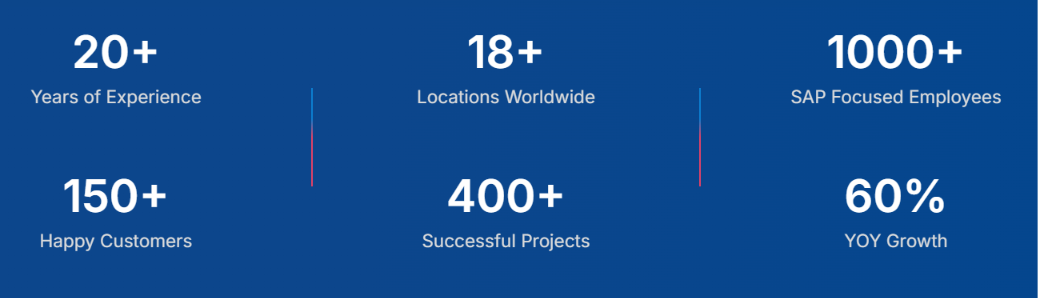
\includegraphics[width=12cm]{Figures/1.png}
    \caption{Cognitus Corporation --- Global Footprint}
    \label{fig:cognitus_global}
\end{figure}

\noindent
Cognitus operates across more than 18 global offices, with its headquarters in the United States and a strategic delivery center in Tangier, Morocco. The company serves over 150 enterprise clients, employs more than 1{,}000 SAP-focused specialists, and has successfully delivered over 400 SAP projects. Its model blends on-shore, off-shore, and nearshore delivery, offering clients both cost efficiency and cultural alignment across time zones.

\subsection{Cognitus Tangier --- Global Delivery and Support Center}

\begin{figure}[H]
    \centering
    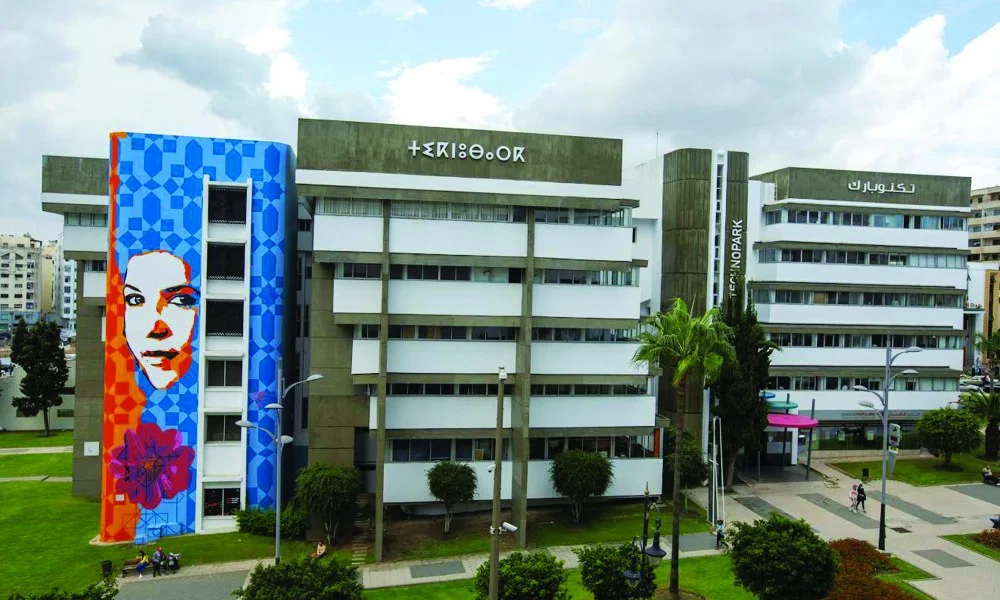
\includegraphics[width=12cm]{Figures/technoparcke.png}
    \caption{Cognitus Tangier --- Technopark, Avenue Mohammed V}
    \label{fig:technoparcke}
\end{figure}

Established in 2021, the Cognitus office in Tangier, Morocco serves as the company's Global Delivery and Support Center (GDSC) for the EMEA region and beyond. Strategically located at Technopark, Avenue Mohammed V, Tangier 90000, this center was designed to leverage the multilingual and highly skilled Moroccan talent pool --- capable of operating in French, Arabic, English, Spanish, and Italian --- to deliver seamless support and implementation services across different time zones.

The Tangier GDSC plays a pivotal role within the Cognitus global operations model. It functions as a nearshore hub that bridges the gap between client needs in Europe, the Middle East, Africa, and North America, and the delivery teams responsible for SAP system configuration, ABAP development, WRICEF object construction, testing, and post-go-live support.

Within this center, cross-functional teams collaborate on live SAP projects, supporting clients with S/4HANA implementations and custom extensions. The center embodies Cognitus's philosophy of combining global reach with localized expertise, offering clients the responsiveness and cultural alignment of a nearshore model with the cost efficiency typically associated with offshore delivery.

% ─────────────────────────────────────────────
\subsection{Business Area of Activity}
% ─────────────────────────────────────────────

Cognitus Corporation operates at the intersection of enterprise technology and business transformation, focusing exclusively on the SAP ecosystem. Its business activity is organized around four major pillars that together cover the full lifecycle of an SAP program:

\begin{itemize}
    \item \textbf{SAP Implementation \& Transformation:} End-to-end delivery of SAP programs, from initial assessment and blueprint design through go-live and hypercare. Cognitus specializes in \textit{RISE with SAP} (private cloud migrations) and \textit{GROW with SAP} (public cloud adoption for mid-market), leveraging pre-built industry templates to accelerate project timelines significantly.

    \item \textbf{Proprietary Accelerator Assets:} Cognitus distinguishes itself through a suite of SAP-endorsed, AI-enabled software products, including:
    \begin{itemize}
        \item \textit{CIS-GovCon} --- a government contracting compliance solution aligned with DCAA, DCMA, FAR, and CAS regulations;
        \item \textit{Contract Lifecycle Management (CLM)} --- an AI-powered tool automating contract authoring, approval, and monitoring;
        \item \textit{Data Migration Accelerator} --- a low-code, AI-assisted platform for migrating legacy data to S/4HANA;
        \item \textit{Real-Time Billing} --- an accelerator for project-based billing and revenue recognition.
    \end{itemize}

    \item \textbf{Application Management Services (AMS):} 24/7 system support, proactive optimization, basis administration, and performance monitoring for clients already on SAP, through on-shore, off-shore, and nearshore delivery models.

    \item \textbf{Strategic Consulting:} Assessment services, M\&A integration technology roadmaps, digital transformation strategy, and organizational change management aligned to SAP programs.
\end{itemize}

\textbf{Industries Served.}
Cognitus concentrates on sectors characterized by high operational complexity and regulatory requirements:

\begin{itemize}
    \item \textbf{Aerospace \& Defense} --- Government contracting, DCAA/DCMA compliance, MRP;
    \item \textbf{Manufacturing} --- Supply chain optimization, production planning, plant maintenance;
    \item \textbf{Life Sciences} --- Serialization, quality management, regulatory traceability;
    \item \textbf{Energy, Oil \& Gas} --- Asset management, project systems, real-time billing;
    \item \textbf{Professional Services} --- Project accounting, CLM, resource management;
    \item \textbf{Consumer Products} --- Demand planning, distribution, trade promotions;
    \item \textbf{Public Sector} --- Federal financials, grants management, GovCon compliance.
\end{itemize}

\textbf{Notable Clients.}
Among Cognitus's reference clients, several high-profile success stories illustrate the depth and speed of its delivery approach:

\begin{itemize}
    \item \textbf{Boom Supersonic} --- Implemented SAP S/4HANA in under three weeks to meet commercialization and regulatory compliance requirements;
    \item \textbf{Phlow Corporation} --- Adopted RISE with SAP to overcome siloed operations and stringent pharmaceutical regulatory requirements;
    \item \textbf{SunnySky Products} --- Standardized multi-site operations using SAP S/4HANA Public Cloud via the GROW with SAP program;
    \item \textbf{Volumetric Building Companies} --- Completed a full ERP modernization in three months using GROW with SAP Fast.
\end{itemize}

% ─────────────────────────────────────────────
\subsection{Enterprise Resource Planning (ERP)}
% ─────────────────────────────────────────────

\subsubsection{What is an ERP System?}

An \textbf{Enterprise Resource Planning (ERP)} system is an integrated suite of software applications designed to manage and automate an organization's core business processes across a single, unified platform. Rather than maintaining isolated systems for finance, procurement, human resources, manufacturing, and logistics, an ERP brings all these functions under one shared database and one coherent process model, enabling real-time visibility, consistent data, and end-to-end process automation across the enterprise.

The fundamental value proposition of an ERP system rests on three pillars:

\begin{enumerate}
    \item \textbf{Integration:} All business modules share a single source of truth. A sales order automatically triggers inventory checks, production planning, procurement, and financial accounting entries --- without any manual re-entry of data.
    \item \textbf{Standardization:} ERP systems enforce best-practice process models (often called \textit{business blueprints}) that align internal workflows with industry standards, reducing errors and audit risk.
    \item \textbf{Real-Time Visibility:} Decision-makers at all levels gain instant access to consolidated operational data, enabling faster and better-informed decisions.
\end{enumerate}

\begin{figure}[H]
    \centering
    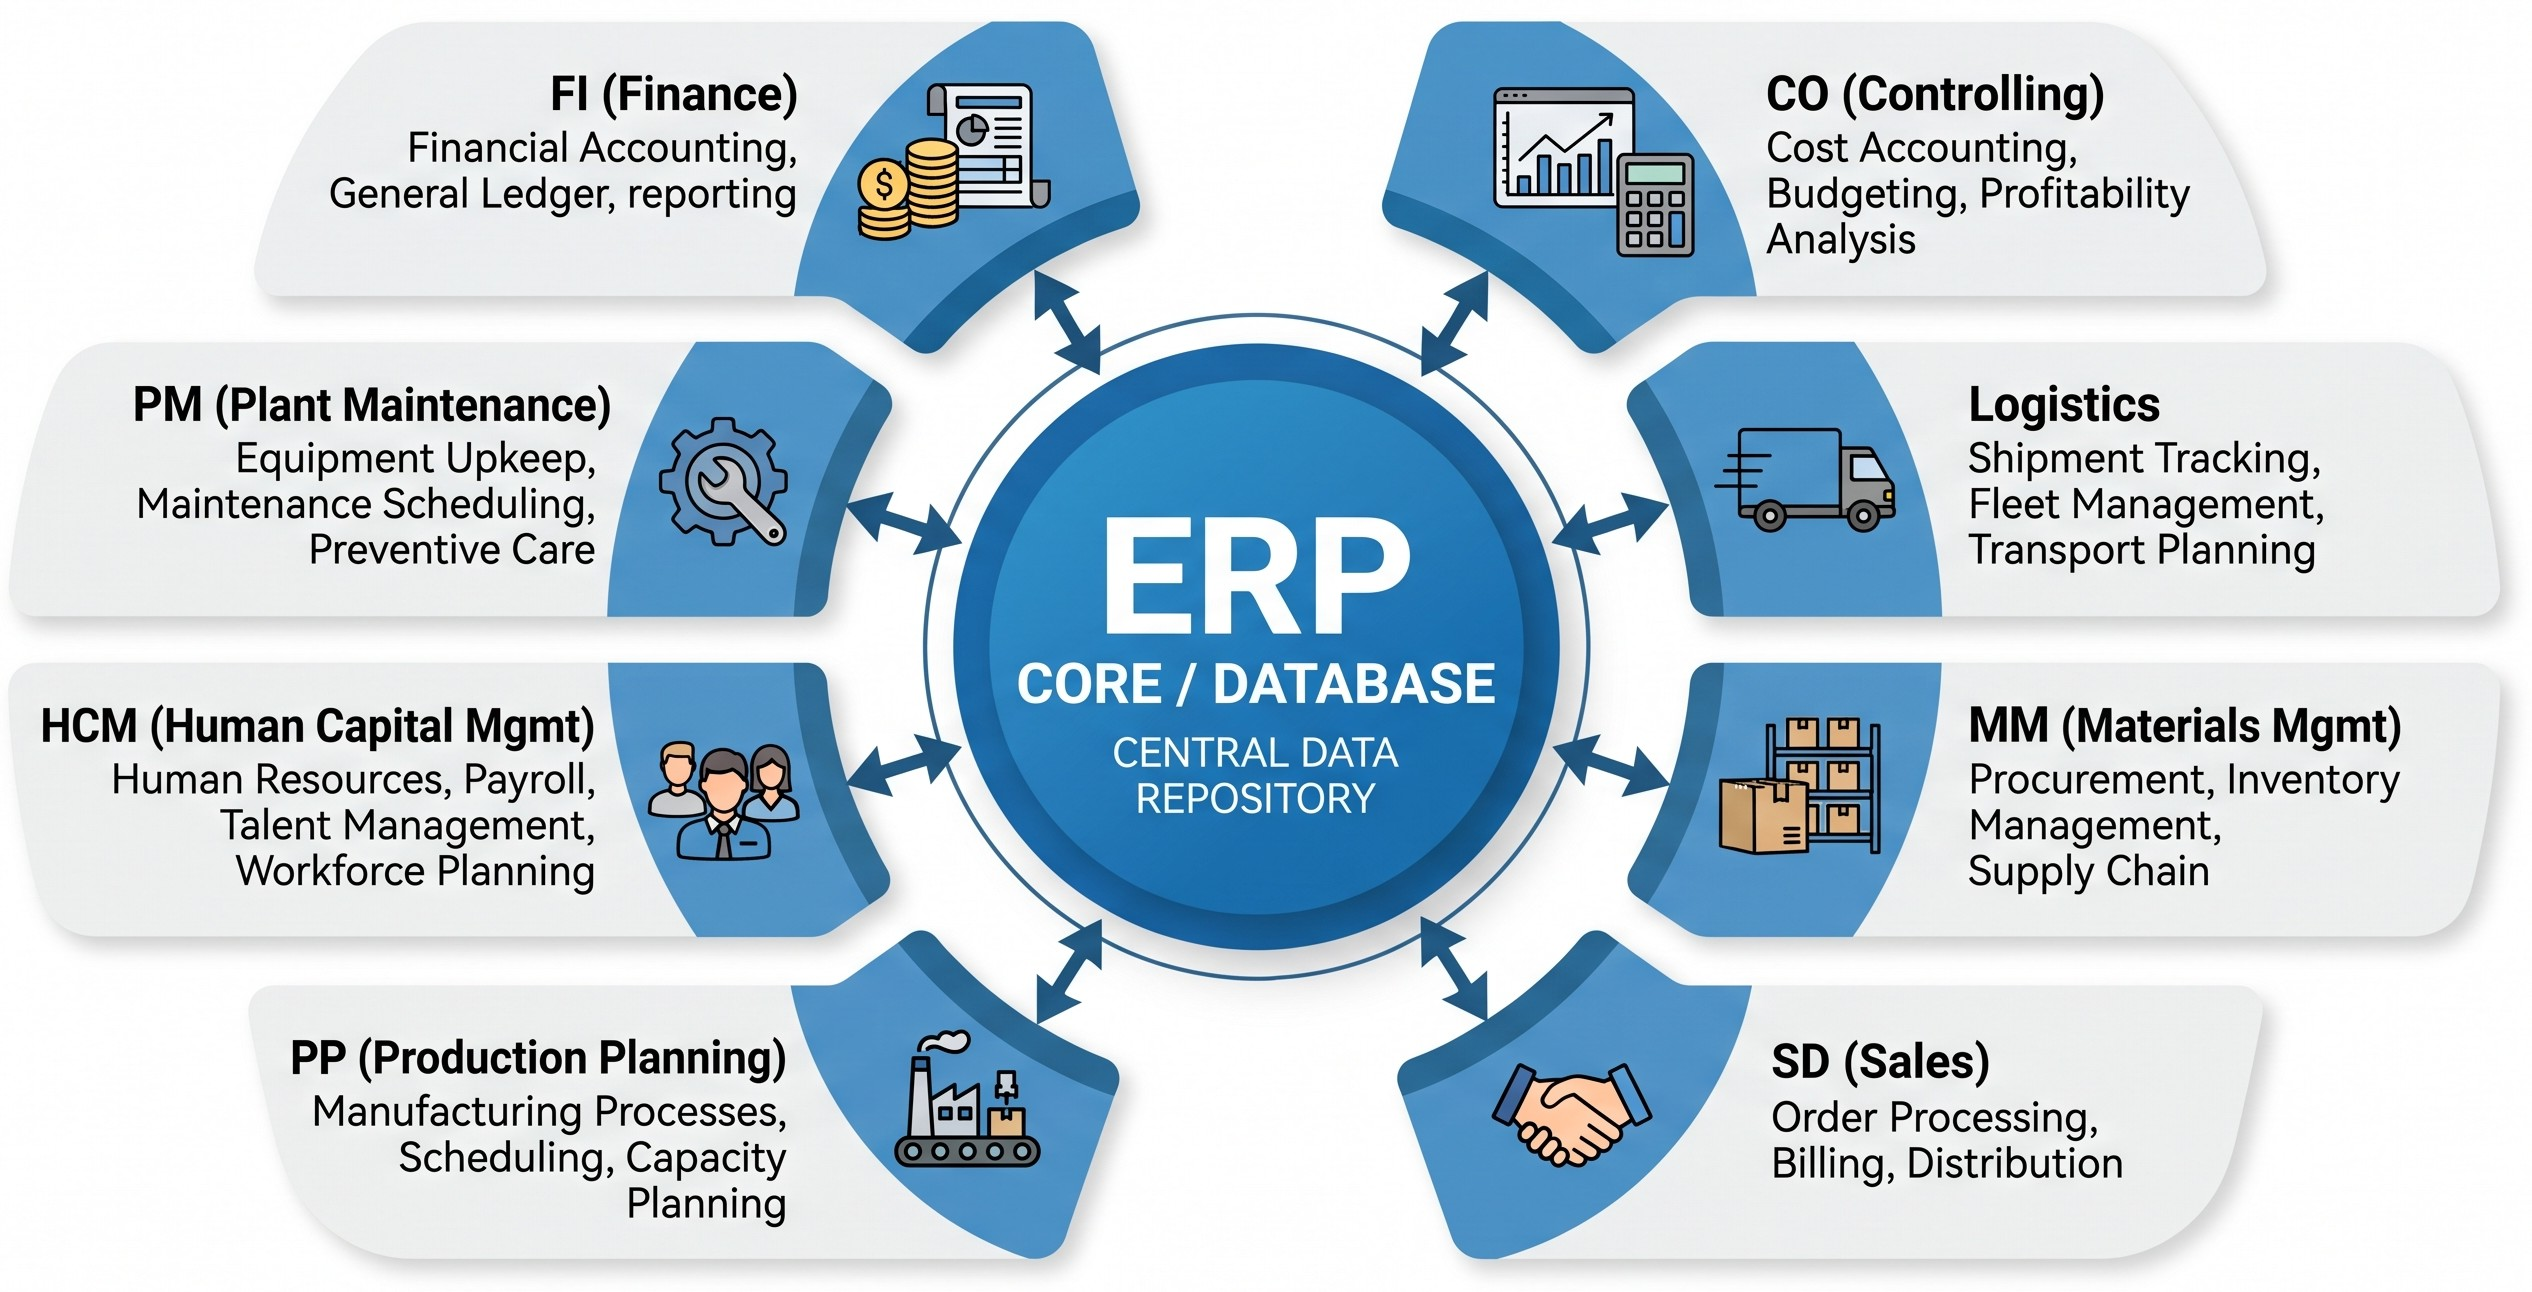
\includegraphics[width=15cm]{Figures/erp_modules.jpg}
    \caption{ERP System --- Integrated Business Module Architecture}
    \label{fig:erp_diagram}
\end{figure}

Modern ERP systems have evolved significantly since their origins in the 1960s--1970s. Early \textit{Material Requirements Planning (MRP)} systems focused solely on manufacturing inventory. The concept expanded in the 1990s into full \textit{ERP} suites covering the entire enterprise, and has since continued to evolve toward cloud-native, AI-augmented platforms capable of processing massive transactional volumes in real time.

In the context of this project, the ERP system at stake is the \textbf{SAP Human Capital Management (HCM)} module, which manages the organization's entire people-related data: employee master records, organizational structure, positions, and job offers. The web recruitment platform developed during this internship consumes and produces data within this SAP HCM layer through standard APIs.

% ─────────────────────────────────────────────
\subsection{SAP --- Systems, Applications, and Products}
% ─────────────────────────────────────────────

\subsubsection{SAP S/4HANA}

\textbf{SAP S/4HANA} is SAP's next-generation ERP suite, built natively on the \textbf{SAP HANA in-memory database}. Unlike its predecessor SAP ECC, S/4HANA delivers real-time transactional analytics, a simplified data model, and a modern web-based experience through \textbf{SAP Fiori}. It covers all core enterprise functions through dedicated modules --- notably \textbf{HCM} (Human Capital Management) for personnel administration, organizational management, and recruitment, which is the module at the heart of this project.

\subsubsection{SAP Business Technology Platform (BTP)}

\textbf{SAP BTP} is SAP's cloud-native \textit{Platform-as-a-Service (PaaS)}, designed to integrate, extend, and build applications across the SAP ecosystem. It unifies four capability areas: \textbf{Database \& Data Management} (HANA Cloud, Datasphere), \textbf{Analytics} (SAP Analytics Cloud), \textbf{Application Development \& Automation} (CAP, SAP Build), and \textbf{Integration} (SAP Integration Suite, API Management).

\subsubsection{ABAP and the RESTful Application Programming Model (RAP)}

\textbf{ABAP} (\textit{Advanced Business Application Programming}) is SAP's proprietary programming language, in use since the early 1980s. Its modern cloud-ready form is the \textbf{ABAP RESTful Application Programming Model (RAP)}, which structures development mainly in three clean layers:

\begin{figure}[H]
    \centering
    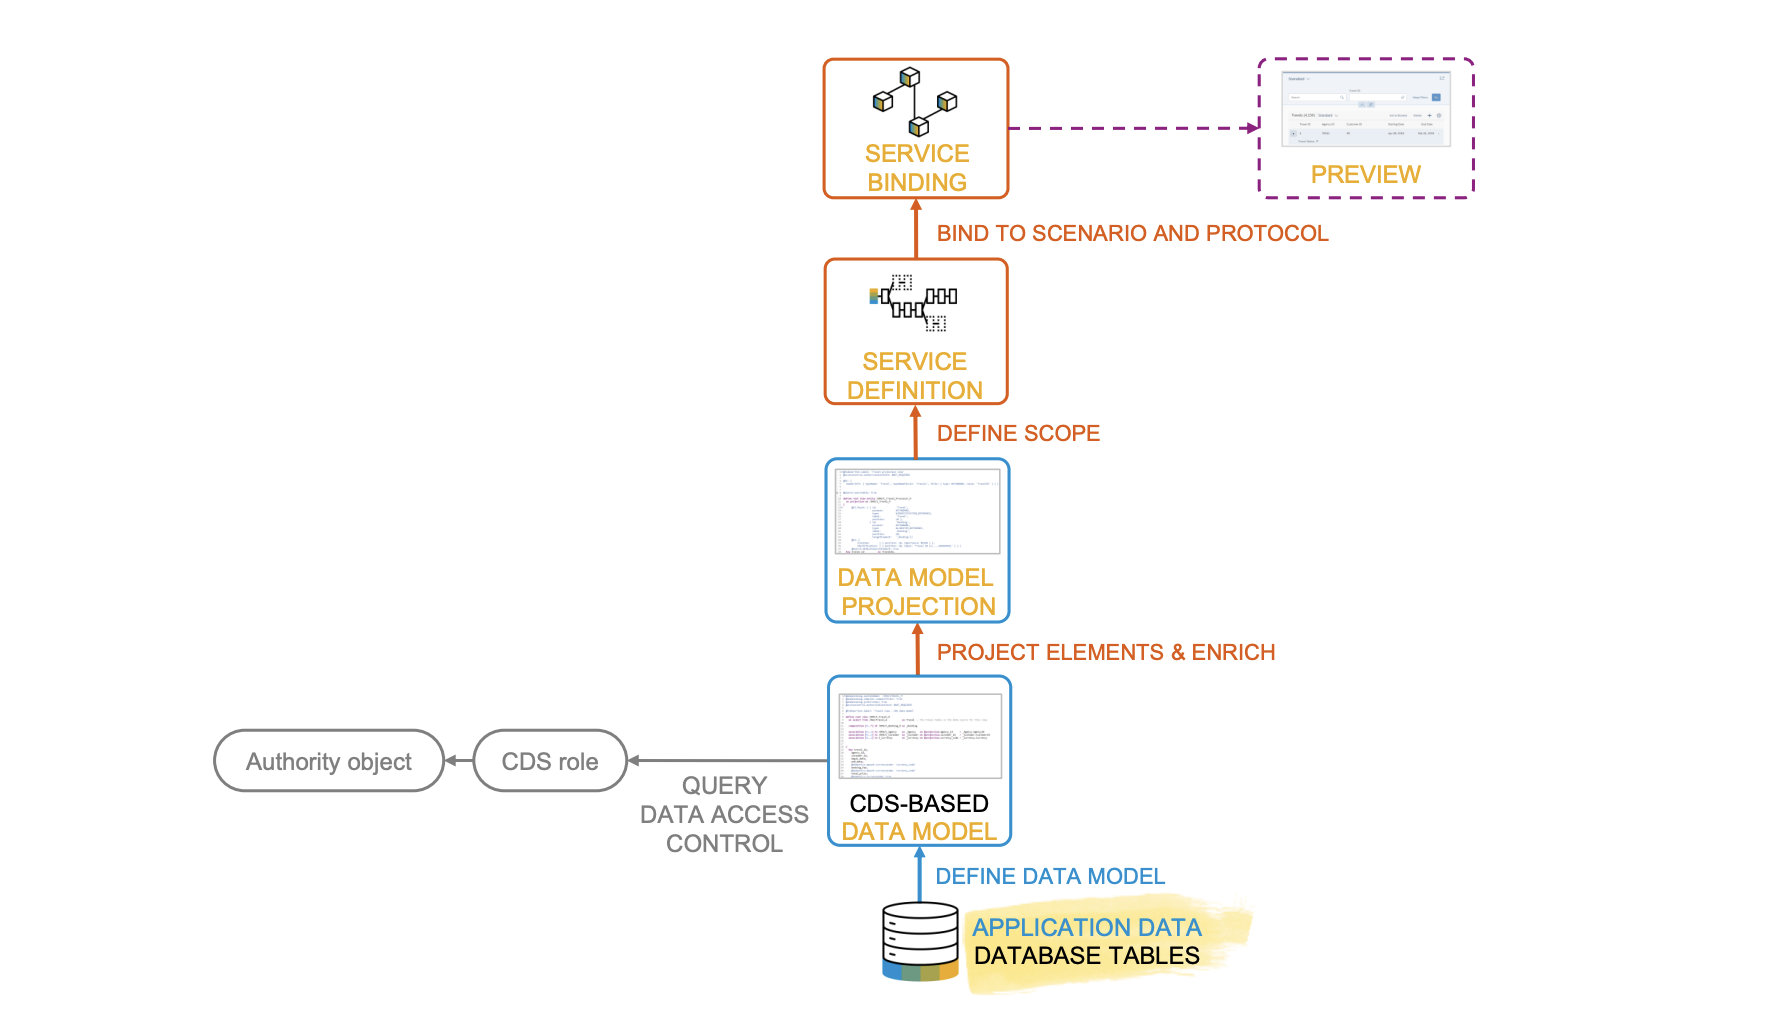
\includegraphics[width=13cm]{Figures/Screenshot-7.png}
    \caption{ABAP RAP --- Layered Architecture}
    \label{fig:rap_architecture}
\end{figure}

\begin{enumerate}
    \item \textbf{CDS View Entities} --- define the data model directly on the HANA database;
    \item \textbf{Behavior Definition (BDEF)} --- specify allowed operations (CRUD, custom actions, business logic) in ABAP;
    \item \textbf{Service Definition \& Binding} --- expose entities as \textbf{OData V4} endpoints consumable by web apps, Fiori, or mobile.
\end{enumerate}

% ─────────────────────────────────────────────
\subsection{Internship Overview}
\label{subsec:internship_overview}
% ─────────────────────────────────────────────

This section provides a structured overview of the technical internship carried out at Cognitus Corporation. It situates the project within the academic curriculum of the INPT, outlines the administrative and supervisory framework governing the internship, defines the core technical objectives of the assignment, and details the project planning, governance methodology, and technical ramp-up undertaken during this two-month immersion.

\subsubsection{Internship Framework}
\label{subsubsec:internship_framework}

The internship was conducted as the mandatory engineering initiation and technical internship (\textit{Stage INE1}) for the ASEDS program at the INPT, Rabat, under the auspices of the \textit{Agence Nationale de R\'eglementation des T\'el\'ecommunications} (ANRT). 

For me, this experience represented my very first professional internship and my initial immersion into the world of enterprise information systems and Enterprise Resource Planning (ERP). Carried out on-site (\textit{Pr\'esentiel}) at the Cognitus Global Delivery and Support Center (GDSC) in Technopark, Tangier, the internship spanned two months, from \textbf{June 15, 2026, to August 15, 2026}: eight weeks of work followed by a closure week.

All contractual, institutional, and organizational modalities were formalized in the official internship agreement (\textit{Convention de stage}). Table~\ref{tab:convention_stage} summarizes the primary administrative parameters of this engagement.

\begin{table}[H]
    \centering
    \begin{tabular}{|m{5cm}|m{9.5cm}|}
        \hline
        \textbf{Item / Field} & \textbf{Specification / Details} \\
        \hline
        \textbf{Host Enterprise} & Cognitus Corporation --- EMEA GDSC (Tangier, Morocco) \\
        \hline
        \textbf{Signatory Representative} & \textbf{Mr.\ Mohamed Reghioui} \newline \textit{Function:} General Manager EMEA \newline \textit{Email:} \href{mailto:mreghioui@cognitus.com}{mreghioui@cognitus.com} \newline \textit{Phone:} +212 (0) 661 93 99 35 \\
        \hline
        \textbf{Industrial Supervisor} & \textbf{Mr.\ Karim A\"it Alla} \newline \textit{Function:} Technical Lead \newline \textit{Email:} \href{mailto:kaitalla@cognitus.one}{kaitalla@cognitus.one} \newline \textit{Phone:} +212 (0) 611 66 58 81 \\
        \hline
        \textbf{Official Assignment Title} & \textit{D\'eveloppement des extensions pour les impl\'ementations SAP} (Development of Extensions for SAP Implementations) \\
        \hline
        \textbf{Internship Period} & June 15, 2026 -- August 15, 2026 (2 months: 8 weeks of work and a closure week) \\
        \hline
        \textbf{Working Modality} & On-site (\textit{Pr\'esentiel}) at Technopark Tangier \\
        \hline
        \textbf{Core Scope \& Missions} & 
        $\bullet$~Comprehensive understanding of enterprise ERP architecture and business workflows; \newline
        $\bullet$~Acquisition of foundational ABAP development and SAP Fiori UI concepts; \newline
        $\bullet$~Understanding, design, and construction of WRICEF objects (Workflows, Reports, Interfaces, Conversions, Enhancements, and Forms). \\
        \hline
    \end{tabular}
    \caption{Internship Agreement Administrative Specifications (\textit{Convention de stage})}
    \label{tab:convention_stage}
\end{table}

\subsubsection{Project Objectives (\textit{Objectifs du projet de stage})}
\label{subsubsec:project_objectives}

Within the broader scope of developing custom extensions for SAP implementations, the specific project assigned to me was titled: \textbf{``Design and Implementation of an Intelligent Talent Acquisition and Employee Administration System Using SAP BTP, ABAP RAP, and Artificial Intelligence''}. 

Recruitment and personnel onboarding are among the most critical operational pillars of enterprise Human Capital Management (HCM). However, traditional enterprise recruitment pipelines face significant challenges: corporate recruiters are frequently overwhelmed by high volumes of incoming applications, manual resume screening is notoriously labor-intensive and subjective, and legacy SAP GUI transaction screens are ill-suited for external candidates and modern mobile-first HR users.

To solve this dilemma, the project sought to bridge the gap between a modern, consumer-grade candidate experience and the enterprise-grade SAP back-end through six core objectives:

\begin{itemize}
    \item \textbf{SAP HCM Data Modeling via ABAP RAP:} Construct Core Data Services (CDS) view entities defining the fundamental HR data models (Organizational Units, Job Positions, Recruitment Job Offers, and Candidate Profiles) directly on the SAP HANA database layer.
    
    \item \textbf{Business Logic \& Behavior Implementation:} Define transactional behavior definitions (BDEF) in ABAP Cloud to enforce business rules, automated determinations, data validations, and state transitions across the candidate lifecycle.

    \item \textbf{Secure OData V4 API Exposure:} Expose the RAP business entities through SAP Service Definitions and Service Bindings as standard OData V4 RESTful APIs, facilitating seamless, decoupled communication with external web applications.

    \item \textbf{AI-Powered Resume Analysis \& Candidate Scoring:} Integrate an intelligent AI screening service capable of parsing semi-structured CV documents (PDF, Word, or text), extracting candidate competencies and work histories, and automatically calculating a rubric-based match score against the requirements of the job.

    \item \textbf{Decoupled External Web Portal:} Build an intuitive, responsive web portal where candidates can browse openings, submit applications, and track their progress without any direct access to the SAP backend, while recruiters review and rank the candidates in an SAP Fiori cockpit.

    \item \textbf{WRICEF Construction \& Clean Core Compliance:} Implement the required WRICEF objects (Interfaces, Reports, Enhancements) while adhering to SAP's \textit{Clean Core} principles to preserve system upgradability.
\end{itemize}

\subsubsection{Project Planning and Management}
\label{subsubsec:project_planning}

To ensure the successful delivery of an enterprise-grade cloud extension within the two-month internship timeframe, this project adopted a rigorous engineering management framework. This structure integrated an intensive preliminary training curriculum on SAP Learning, learning about HCM and S/4HANA, and an Agile development lifecycle governed by the Scrum framework.

% ══════════════════════════════════════════════
\paragraph{A. Formation et Mont\'{e}e en Comp\'{e}tences --- Technical Training \& Upskilling}
% ══════════════════════════════════════════════

Entering the SAP enterprise ecosystem required a dedicated, intensive preparation phase. The first weeks of the internship were dedicated to technical upskilling on \textbf{SAP Learning}~\cite{sap_learning}, through three official courses totalling about \textbf{41 hours} (4~h for BTP100, 17~h for S4D400, and 20~h for S4D437) with hands-on exercises in the SAP BTP ABAP Environment, alongside an exploration of SAP and Human Capital Management domain concepts:

\begin{enumerate}

    \item \textbf{Exploring SAP Business Technology Platform (BTP100)} \textit{--- Level: Beginner}

    \textit{Core Curriculum:} Covered the foundational multi-cloud architecture of SAP BTP, core infrastructure providers, security and identity provisioning, runtime environments --- Cloud Foundry, Kyma, and ABAP Cloud --- and side-by-side extension paradigms.

    \textit{Direct Project Value:} Provided the architectural blueprint to design the recruitment platform as a decoupled cloud application on SAP BTP, strictly adhering to SAP's \textbf{Clean Core} strategy by leaving standard ERP core tables untouched.

    \item \textbf{Learning Basic ABAP Programming (S4D400)} \textit{--- Level: Beginner}

    \textit{Core Curriculum:} Covered the basics of ABAP programming in the SAP BTP ABAP Environment: data types and internal tables, SQL access to database tables, modern expressions such as \texttt{VALUE}, \texttt{CORRESPONDING}, and \texttt{FILTER}, object-oriented modularization with classes and interfaces, and the Eclipse-based ABAP Development Tools.

    \textit{Direct Project Value:} Established the programmatic foundation required to write clean, type-safe business logic, custom calculations, and validation routines.

    \item \textbf{Building Transactional Apps with the ABAP RESTful Application Programming Model (S4D437)} \textit{--- Level: Advanced}

    \textit{Core Curriculum:} Delivered deep mastery of Core Data Services view entities, transactional Behavior Definitions, the RAP interaction phase and save sequence, transactional draft handling, custom business actions, determinations, validations, dynamic feature control, and publishing OData V4 Web API and UI services.

    \textit{Direct Project Value:} Formed the functional and transactional backbone of the platform, enabling robust draft state management for incomplete requisitions, fine-grained entity validation, atomic employee onboarding commits, and seamless API exposure for both the React web portal and the Python AI microservice.

    \item \textbf{SAP HCM Domain Research \& Organizational Modeling}

    In addition to technical frameworks, substantial self-directed research was conducted into standard \textbf{SAP Human Capital Management} business processes. This covered the structural relationship between \textbf{Organizational Units} and \textbf{Positions} --- enforcing vacancy states: \textit{Vacant}, \textit{Filled}, \textit{Frozen}, and budgeted compensation ceilings --- as well as classical personnel \textbf{Infotypes} for Organizational Assignment, Personal Data, Addresses, and Bank Details.

    \textit{Direct Project Value:} Enabled the reverse-engineering and modernization of standard SAP HCM structures into native CDS data models and informed the design of the atomic onboarding action that generates complete Employee Master Records.

\end{enumerate}

The completion of the courses is recorded in SAP Learning. The BTP100 and S4D400 courses award a course completion badge (Figure~\ref{fig:sap_certificate}), while S4D437 records the completion without a badge. As the learning list shows (Figure~\ref{fig:sap_learning_dashboard}), BTP100 was completed on June 15, 2026, and the S4D400 and S4D437 courses, started during the internship, were formally completed on October 11, 2026.

\begin{figure}[H]
    \centering
    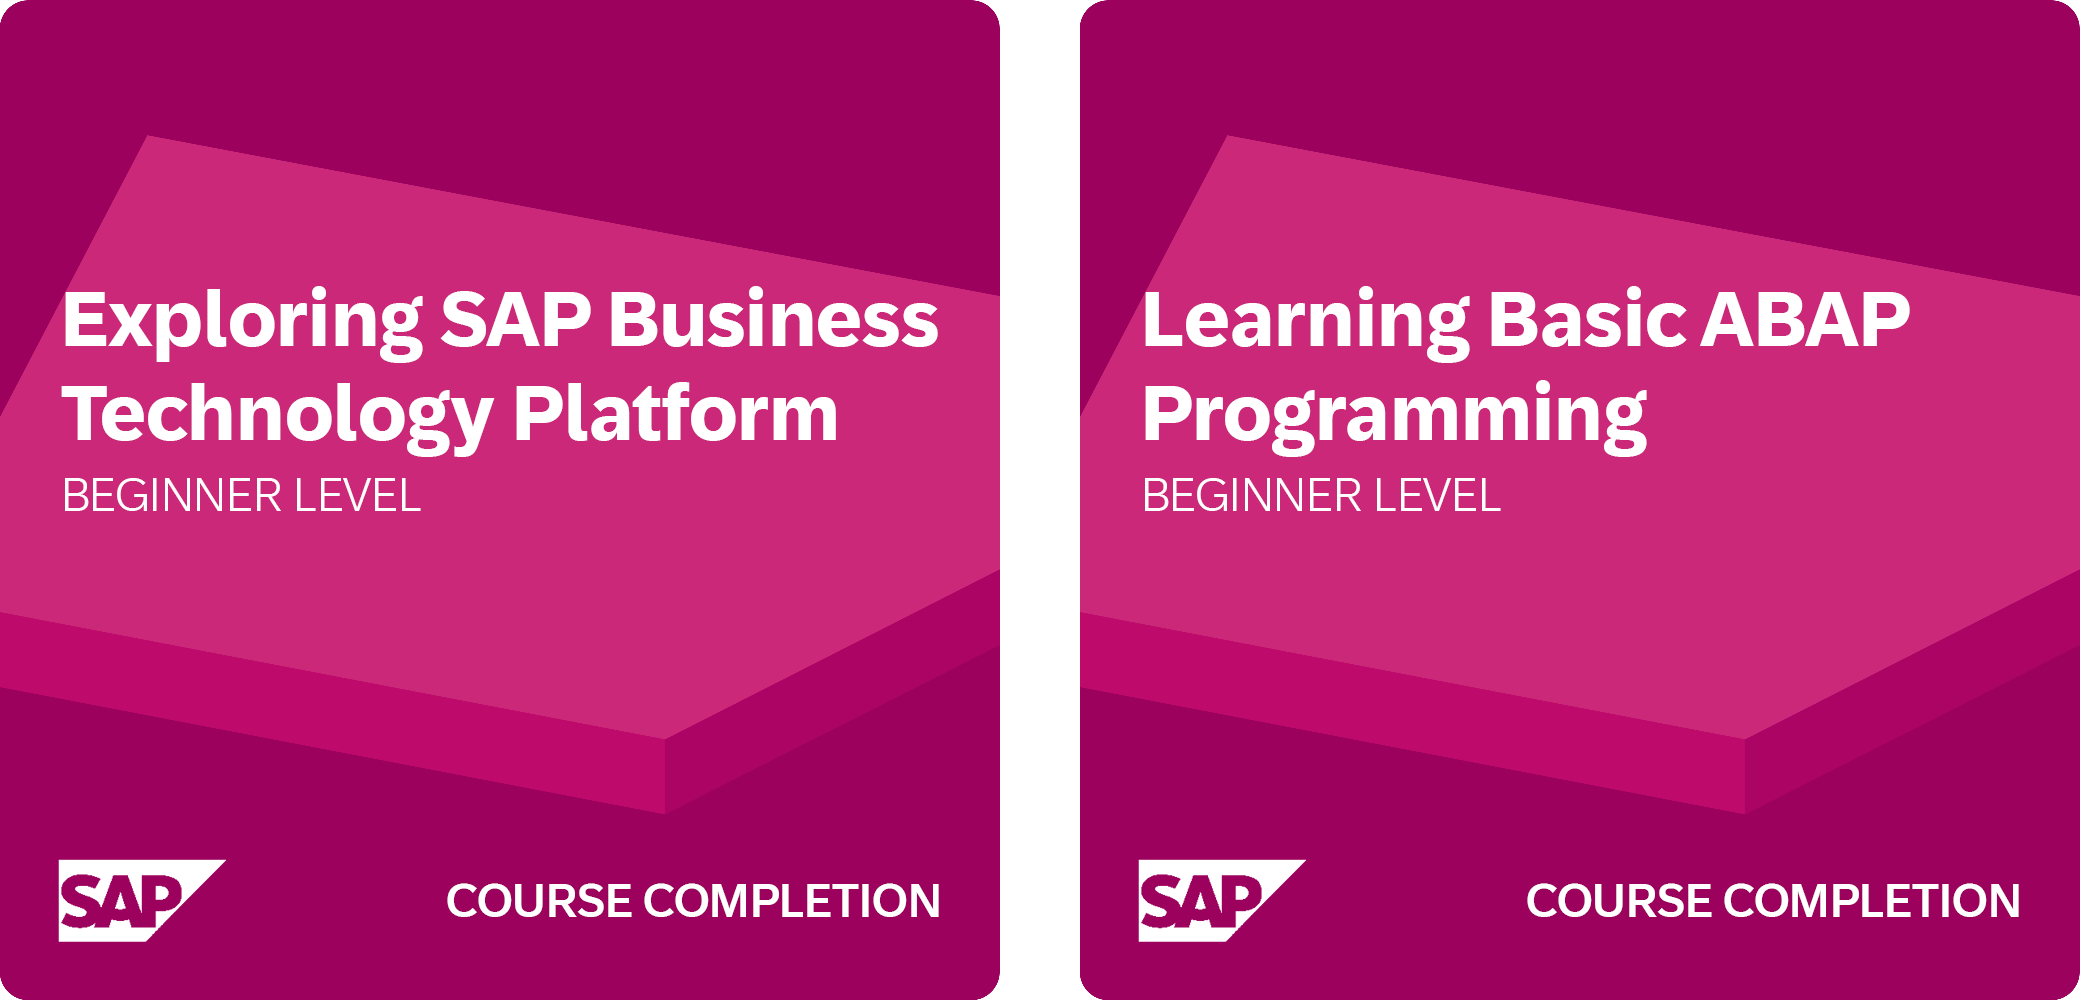
\includegraphics[width=12cm]{Figures/sap_certificate.png}
    \caption{SAP Learning --- Course Completion Badges (BTP100 and S4D400)}
    \label{fig:sap_certificate}
\end{figure}

\begin{figure}[H]
    \centering
    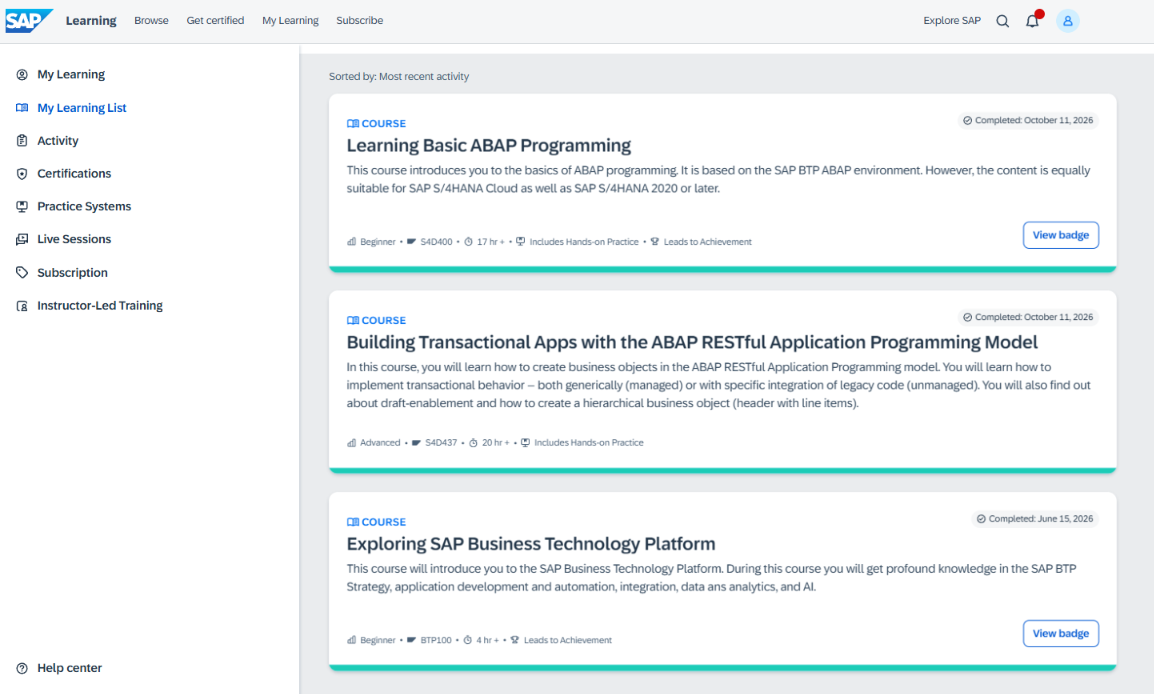
\includegraphics[width=14cm]{Figures/sap_learning_hub_dashboard.png}
    \caption{SAP Learning --- List of Completed Courses}
    \label{fig:sap_learning_dashboard}
\end{figure}

% ══════════════════════════════════════════════
\paragraph{B. Conduite de Projet --- The Scrum Framework}
% ══════════════════════════════════════════════

To manage developmental complexity and foster rapid adaptability, the project was conducted following the \textbf{Scrum Framework}~\cite{scrum_guide}, the premier agile methodology for iterative, high-value product engineering.

\textbf{Foundational Scrum Principles.} Implementing the project under Scrum best practices relied on three foundational pillars:

\begin{itemize}
    \item \textbf{Autonomous, Cross-Functional Execution} --- Rapidly pivoting technical scopes and adapting to architectural feedback through close collaboration between the intern and the industrial supervisor.
    \item \textbf{Iterative Time-Boxed Sprints} --- Organizing the development lifecycle into short, structured two-week iterations facilitating continuous integration, regular testing, and progressive feature delivery.
    \item \textbf{Product Backlog Prioritization} --- Systematically consolidating functional and non-functional requirements into a dynamic, centralized backlog that evolved as technical discoveries were made.
\end{itemize}

\begin{figure}[H]
    \centering
    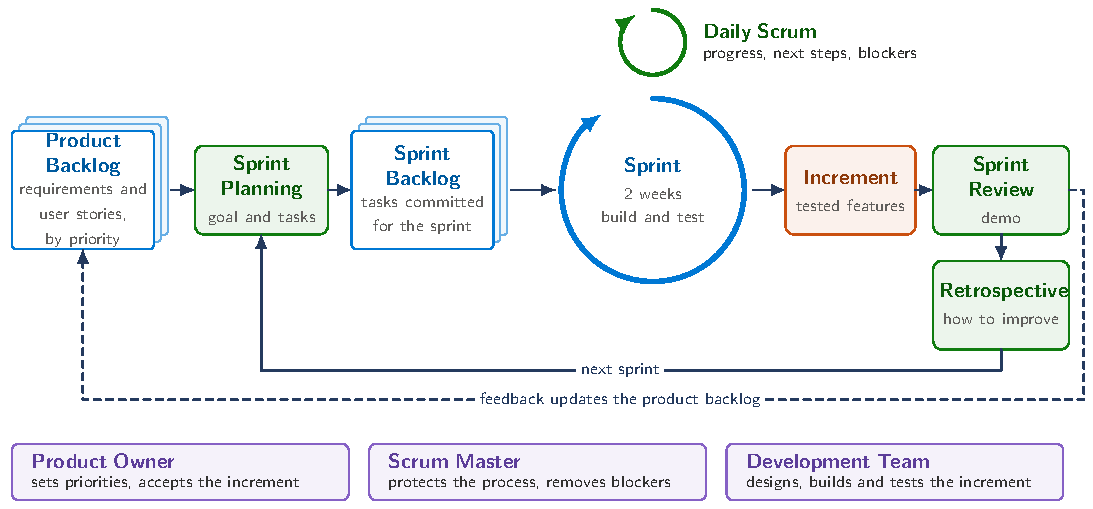
\includegraphics[width=\textwidth]{Figures/scrum_framework.pdf}
    \caption{The Scrum Framework --- Iterative Development Cycle}
    \label{fig:scrum_framework}
\end{figure}

\textbf{Scrum Roles \& Synergy.} The project established clear ownership across the three canonical Scrum roles:

\begin{itemize}
    \item \textbf{Product Owner} --- Represented by the enterprise leadership and Technical Lead, Mr.\ Karim A\"it Alla, acting as the proxy for corporate expectations, resolving requirement ambiguities, and establishing backlog priorities.
    \item \textbf{Scrum Master} --- Ensured rigorous adherence to Agile practices, monitored sprint cadence, eliminated technical roadblocks such as cloud quota allocations and API connectivity issues, and safeguarded project milestones.
    \item \textbf{Development Team} --- Executed autonomously by the intern, Mr.\ Oualid AMTOUT, assuming full technical responsibility for architectural modeling, RAP backend coding, React portal frontend engineering, AI microservice development, and testing.
\end{itemize}

\textbf{Core Scrum Ceremonies.} The iterative lifecycle was punctuated by four essential events:

\begin{itemize}
    \item \textbf{Sprint Planning} --- Conducted at the start of each iteration to decompose user stories from the Product Backlog into discrete technical tasks and commit to sprint goals.
    \item \textbf{Sprint Execution} --- The active engineering phase encompassing CDS data modeling, behavior definition programming, UI development, and API integration.
    \item \textbf{Sprint Review \& Retrospective} --- Concluding demonstrations where working increments were presented to the supervisor, followed by retrospective evaluations to optimize developmental efficiency for subsequent sprints.
    \item \textbf{Backlog Refinement} --- Continuous reassessment and estimation of upcoming user stories to adapt to emerging technical constraints.
\end{itemize}

\textbf{Sprint Plan.} The product backlog was distributed over four two-week sprints, followed by a closure week (Figure~\ref{fig:sprint_plan}). Each sprint had a goal and a set of backlog items taken from the work packages of the Software Development Plan: the first two sprints were devoted to the SAP training and the scoping of the project, the third to the specification and the data model, and the fourth to the integrated prototype, its tests, and its deployment. The backlog items were followed as task lists kept with the project documentation, and the source code was versioned on GitHub.

\begin{figure}[H]
    \centering
    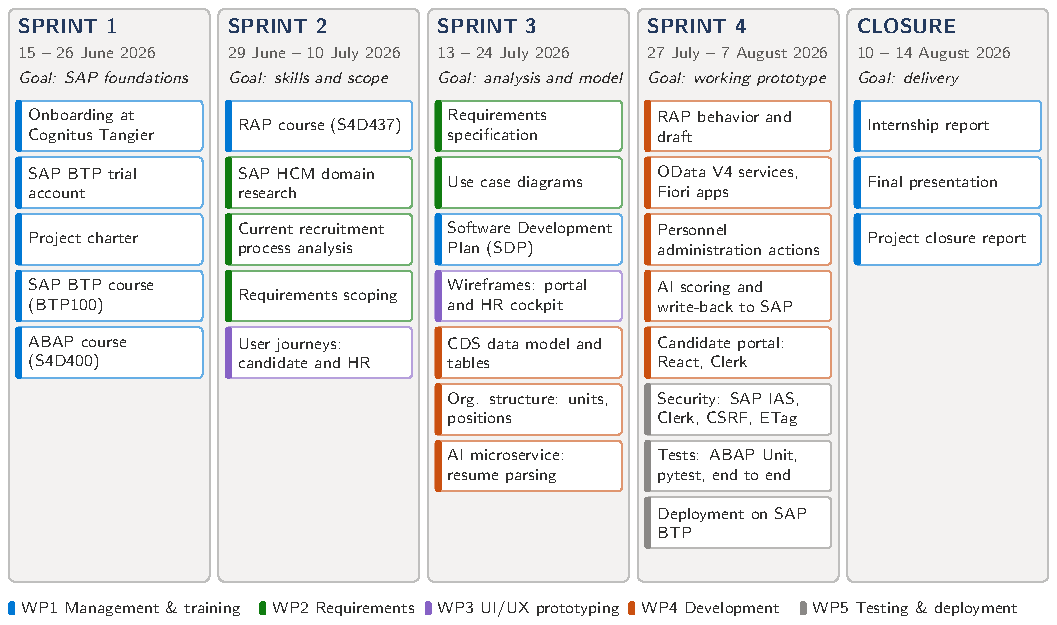
\includegraphics[width=\textwidth]{Figures/sprint_plan.pdf}
    \caption{Sprint Plan --- Product Backlog Distributed over Four Two-Week Sprints}
    \label{fig:sprint_plan}
\end{figure}

% ══════════════════════════════════════════════
\paragraph{C. Gouvernance du Projet --- Formal Governance Artifacts}
% ══════════════════════════════════════════════

Project governance and task monitoring were anchored in two formal enterprise management documents alongside a detailed Gantt schedule:

\begin{itemize}

    \item \textbf{Project Charter:} This document formalizes the context, goal, and objectives of the project, its scope (inclusions and exclusions), the chosen delivery strategy, the stakeholder analysis, the main risks with their mitigation, a preliminary budget and schedule, and the value expected from the solution. Figure~\ref{fig:charte_projet} shows its delivery strategy section, which compares an internal, an external, and a joint delivery.

    \begin{figure}[H]
        \centering
        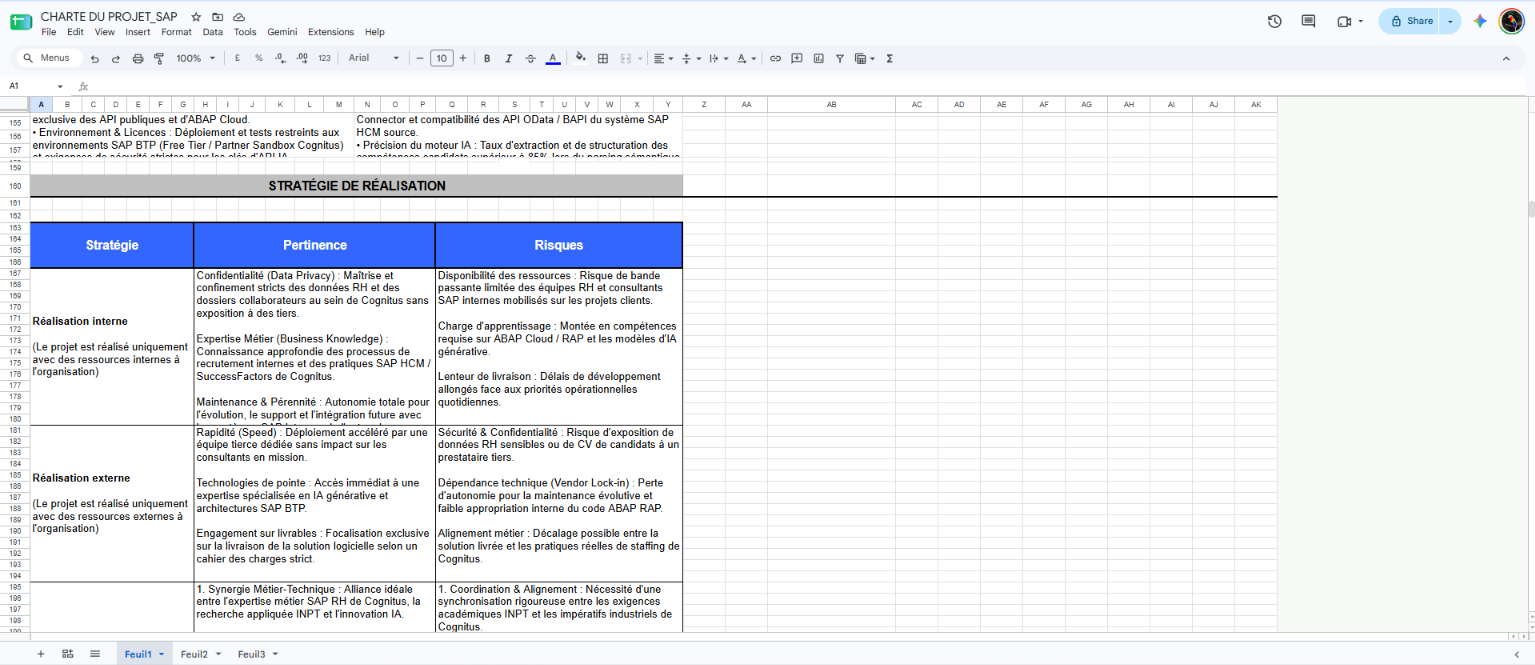
\includegraphics[width=\textwidth]{Figures/charte_projet.png}
        \caption{Project Charter --- Delivery Strategy Section}
        \label{fig:charte_projet}
    \end{figure}

    \item \textbf{Software Development Plan:} The SDP is the operational plan of the project. Its work breakdown structure organizes the work into \textbf{five work packages} (Figure~\ref{fig:sdp_document}):

    \begin{enumerate}
        \item \textbf{WP1 --- Project Management and Training:} project charter, development plan, SAP BTP trial account, SAP courses, internship report, and closure report.
        \item \textbf{WP2 --- Requirements \& Specifications Analysis:} analysis of the current process, SAP HCM recruitment and personnel administration workflows, functional and non-functional requirements, use cases, comparison of language models, and conceptual data model.
        \item \textbf{WP3 --- UI/UX Prototyping:} user journeys, wireframes of the candidate portal and of the HR cockpit, application and onboarding forms, and visual style.
        \item \textbf{WP4 --- Backend \& Frontend Development:} database tables, CDS views, behavior definitions and business objects, OData V4 services, the React candidate portal, and the FastAPI AI microservice.
        \item \textbf{WP5 --- Testing \& Deployment:} unit and integration tests, tests of the recruitment pipeline and of the onboarding, edge cases, end-to-end tests, and deployment on SAP BTP.
    \end{enumerate}

    This report follows the same structure: the analysis of Chapter~\ref{chap:analysis_specifications} and the design of Chapter~\ref{chap:solution_design} cover WP2 and WP3, and the realization and tests of Chapter~\ref{chap:implementation} cover WP4 and WP5.

    \begin{figure}[H]
        \centering
        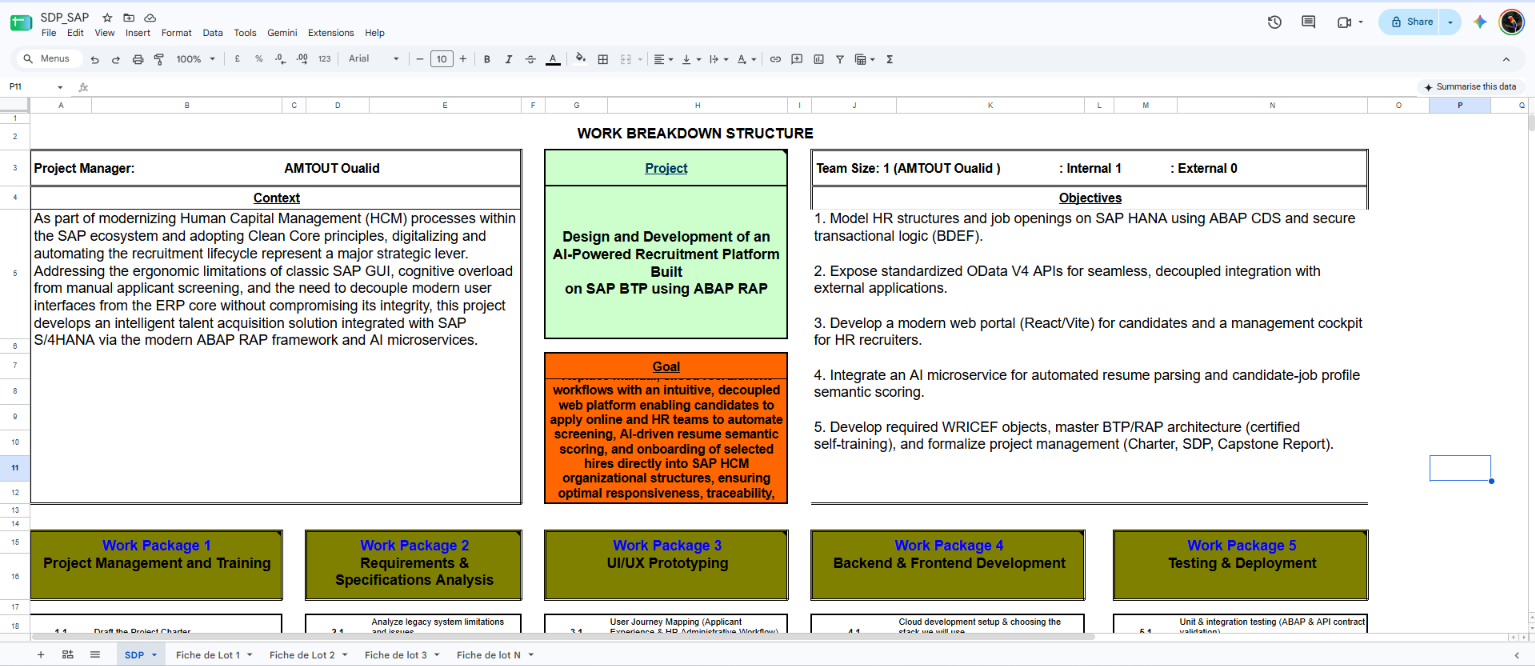
\includegraphics[width=\textwidth]{Figures/sdp_document.png}
        \caption{Software Development Plan --- Work Breakdown Structure}
        \label{fig:sdp_document}
    \end{figure}

\end{itemize}

The main risks identified in the project charter, with their assessment and the measures taken to reduce them, are summarized in Table~\ref{tab:risk_matrix}.

\begin{table}[H]
\centering
\caption{Main Project Risks and Mitigation Measures}
\label{tab:risk_matrix}
\renewcommand{\arraystretch}{1.3}
\setlength{\tabcolsep}{4pt}
\footnotesize
\begin{tabular}{|>{\raggedright\arraybackslash}p{4.0cm}|>{\raggedright\arraybackslash}p{1.3cm}|>{\raggedright\arraybackslash}p{2.0cm}|>{\raggedright\arraybackslash}p{1.85cm}|>{\raggedright\arraybackslash}p{2.35cm}|>{\raggedright\arraybackslash}p{5.25cm}|}
\hline
\textbf{Risk} & \textbf{Impact} & \textbf{Probability} & \textbf{Criticality} & \textbf{Category} & \textbf{Mitigation} \\
\hline
R1. Integration of the three components: OData V4 calls from the React portal (CSRF, ETag, CORS, sessions of the trial account) and write-back of the AI score & High & Medium & High & Technical & Dedicated RAP actions (\texttt{applyToJob}, \texttt{setAIEvaluation}), development proxy for the portal, and early end-to-end tests. \\
\hline
R2. Quality of the AI evaluation: incomplete parsing of heterogeneous resumes or wrong assessment of the skills & Medium & Medium & Medium & Functional, AI & Normalized prompts, strict JSON output, score computed in Python, human decision required, and tests on fictitious resumes of different levels. \\
\hline
R3. Confidentiality: exposure of the personal data of candidates or employees & Critical & Low & High & Security, legal & Separate authentication (SAP IAS for HR, Clerk for candidates), HTTPS, fictitious test resumes, and an AI microservice without database. \\
\hline
R4. User adoption: reluctance toward new screens and algorithmic suggestions & Medium & Low & Low & Organizational & Standard SAP Fiori Elements interfaces, screen mockups, and regular demonstrations. \\
\hline
R5. Trial account and schedule: session expiry, limits of the SAP BTP trial account, and risk of exceeding the planned weeks & High & Low & Medium & Planning, infrastructure & Scrum with two-week sprints, prioritized minimum viable product, and regular backup of the code with abapGit and GitHub. \\
\hline
\end{tabular}
\end{table}

% ══════════════════════════════════════════════
\paragraph{D. Planning d'Ex\'{e}cution --- Implementation Schedule \& Gantt Diagram}
% ══════════════════════════════════════════════

The eight weeks of work were organized in four phases, followed by a closure week, as summarized in Table~\ref{tab:implementation_phases}.

\begin{table}[H]
\centering
\caption{Implementation Schedule --- Phases, Timeframes, and Key Milestones}
\label{tab:implementation_phases}
\renewcommand{\arraystretch}{1.4}
\small
\begin{tabular}{|>{\raggedright\arraybackslash}p{2.6cm}|>{\raggedright\arraybackslash}p{2.2cm}|>{\raggedright\arraybackslash}p{9.2cm}|}
\hline
\textbf{Phase} & \textbf{Timeframe} & \textbf{Focus Area \& Key Milestones} \\
\hline
Phase 1: Onboarding \& Training & Weeks 1--4 & Team integration at Technopark Tangier, SAP Learning courses (BTP100, S4D400, S4D437), project charter, and initial requirement scoping. \\
\hline
Phase 2: Analysis \& Data Modeling & Weeks 5--6 & Software Development Plan, requirements and UML use cases, CDS data model, and organizational structure modeling. \\
\hline
Phase 3: Development \& Integration & Weeks 6--7 & RAP behavior definitions, draft handling, OData V4 services, Fiori Elements applications, FastAPI AI microservice, and React candidate portal. \\
\hline
Phase 4: Testing \& Finalization & Week 8 & Unit and end-to-end tests, feature control validation, deployment on SAP BTP, and technical documentation. \\
\hline
Closure & Week 9 & Internship report, presentation, and project closure report. \\
\hline
\end{tabular}
\end{table}

The detailed schedule, with its tasks, dependencies, and milestones, was modeled with \textbf{GanttProject}~\cite{ganttproject}, as illustrated in Figure~\ref{fig:gantt_diagram}.

\begin{figure}[H]
    \centering
    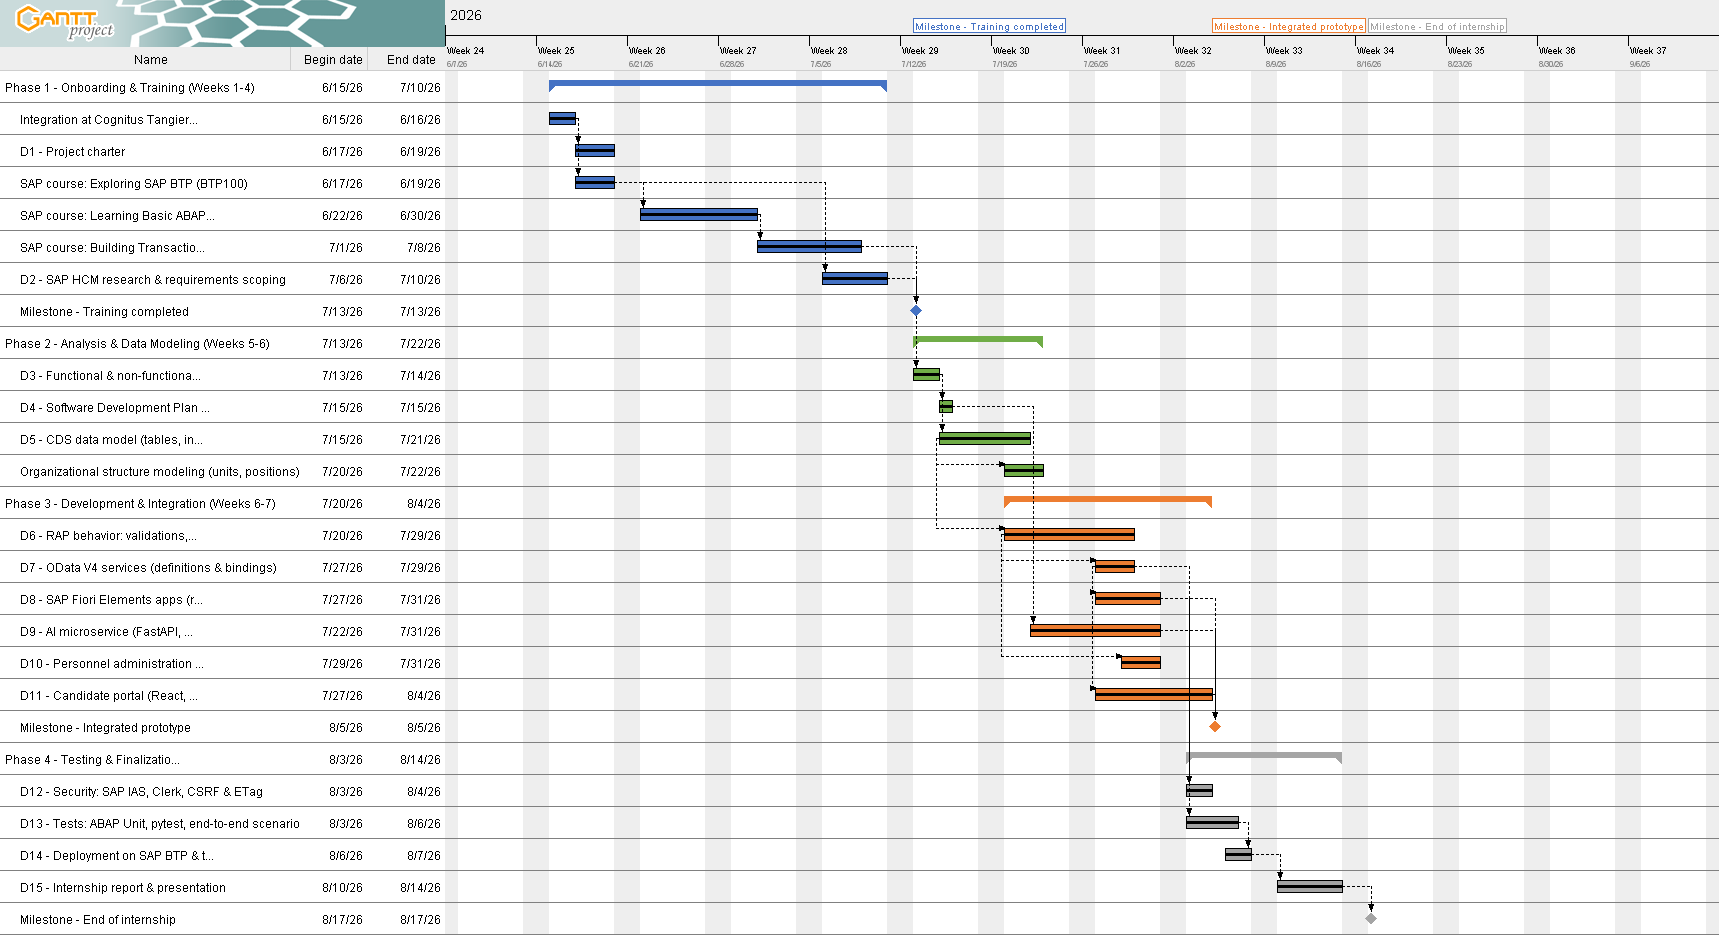
\includegraphics[width=\textwidth]{Figures/Gantt_Diagram.png}
    \caption{Project Planning --- Detailed Gantt Diagram}
    \label{fig:gantt_diagram}
\end{figure}

\newpage

% ─────────────────────────────────────────────
\section*{Conclusion}
\addcontentsline{toc}{section}{Conclusion}
% ─────────────────────────────────────────────

This chapter introduced Cognitus Corporation, a global SAP Gold Partner now part of IBM, and its Tangier Global Delivery and Support Center where this work was carried out. We examined the company's core business areas, key industries, and notable client portfolio, then established the conceptual foundations of ERP systems and the modern SAP technology stack underpinning this project. Finally, we detailed the institutional framework, technical objectives, training curriculum, Scrum-based project governance, and structured implementation schedule that guided the two-month internship. The following chapter presents the project context and objectives in greater detail.
